\hypertarget{ll__move_8c}{
\section{ll\_\-move.c File Reference}
\label{ll__move_8c}\index{ll_move.c@{ll\_\-move.c}}
}


\subsection{Detailed Description}
\begin{Desc}
\item[For internal use only.]
This file contains the implementation of the \hyperlink{group__dbprim__link_ga7}{ll\_\-move()} function, used to move a linked list element to another location within the linked list.\end{Desc}


Definition in file \hyperlink{ll__move_8c-source}{ll\_\-move.c}.

{\tt \#include \char`\"{}dbprim.h\char`\"{}}\par
{\tt \#include \char`\"{}dbprim\_\-int.h\char`\"{}}\par


Include dependency graph for ll\_\-move.c:\begin{figure}[H]
\begin{center}
\leavevmode
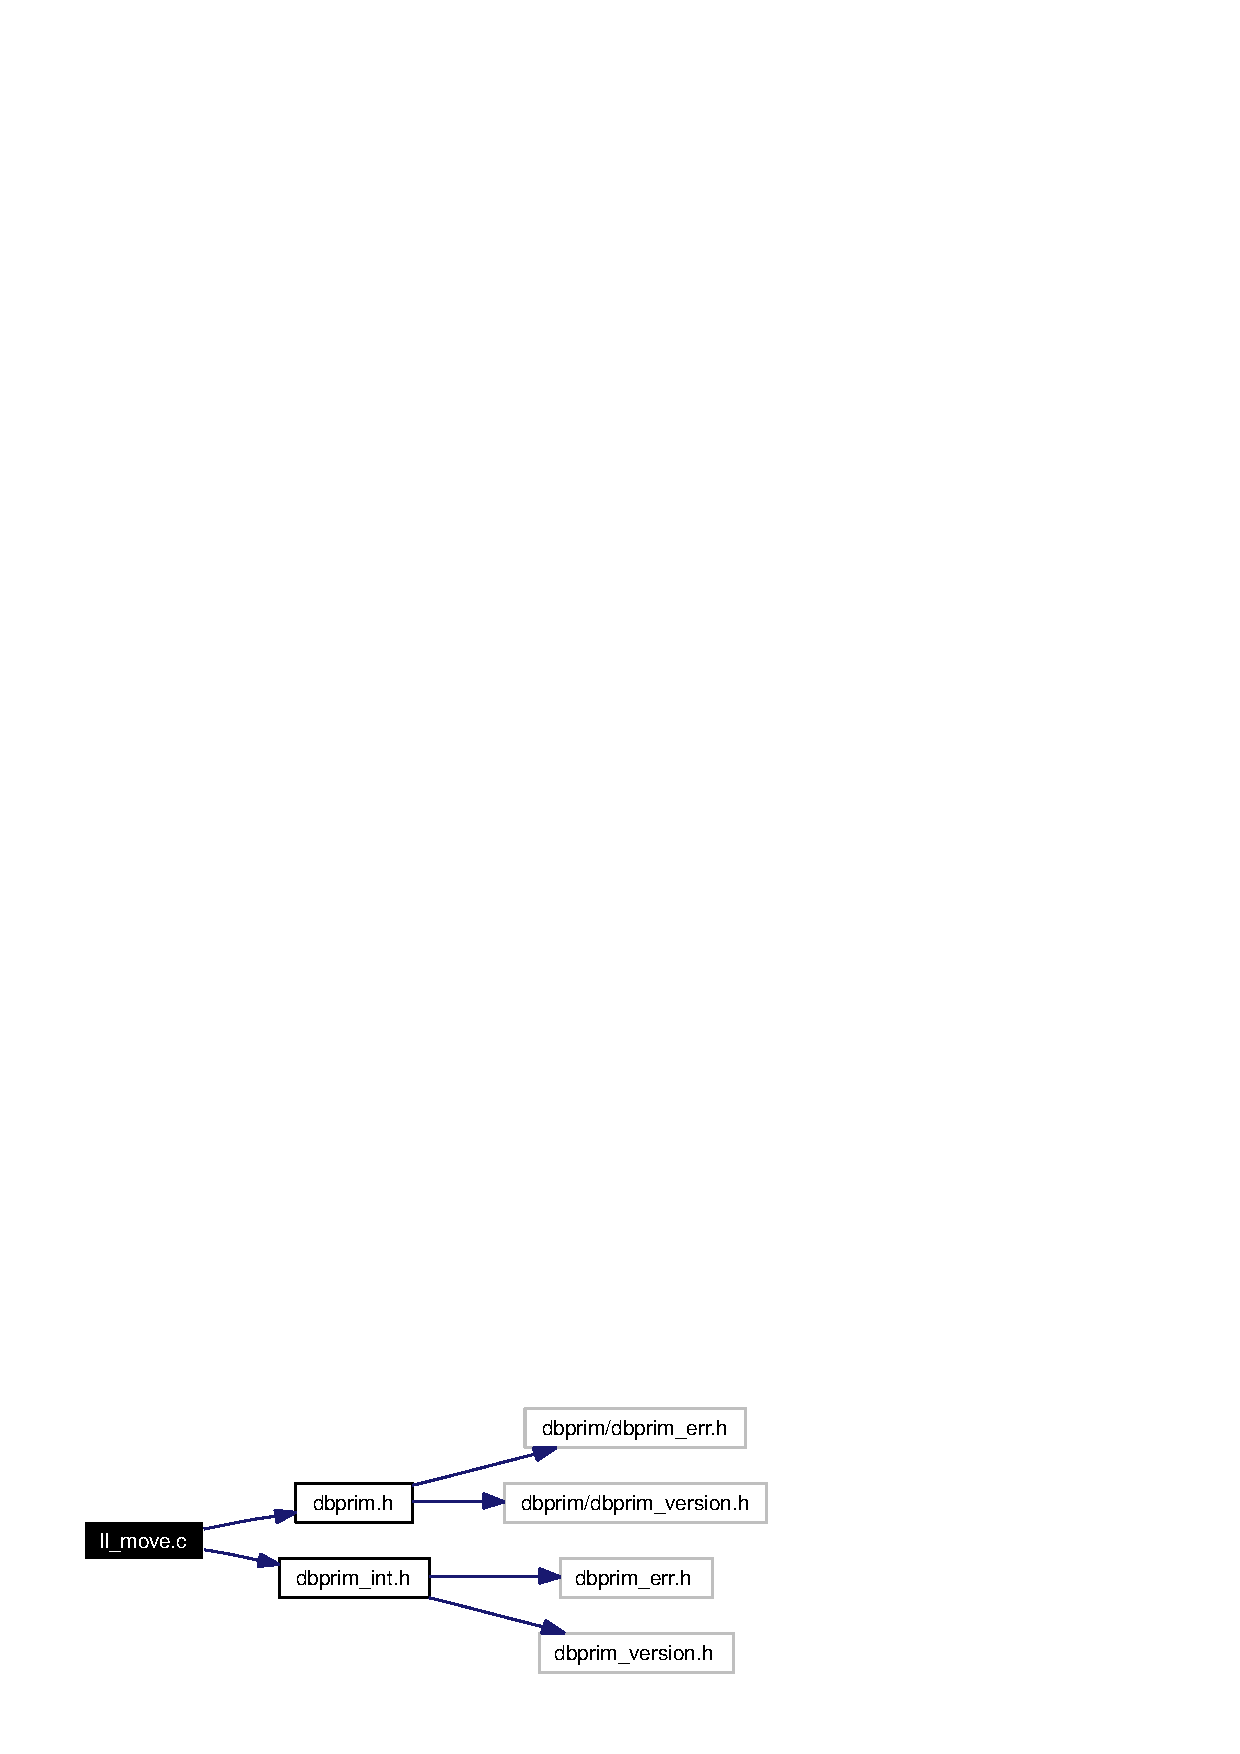
\includegraphics[width=186pt]{ll__move_8c__incl}
\end{center}
\end{figure}
\subsection*{Functions}
\begin{CompactItemize}
\item 
unsigned long \hyperlink{group__dbprim__link_ga7}{ll\_\-move} (\hyperlink{struct__link__head__s}{link\_\-head\_\-t} $\ast$list, \hyperlink{struct__link__elem__s}{link\_\-elem\_\-t} $\ast$new, \hyperlink{group__dbprim__link_ga4}{link\_\-loc\_\-t} loc, \hyperlink{struct__link__elem__s}{link\_\-elem\_\-t} $\ast$elem)
\begin{CompactList}\small\item\em Move an element within a linked list. \item\end{CompactList}\end{CompactItemize}
